\PassOptionsToPackage{unicode=true}{hyperref} % options for packages loaded elsewhere
\PassOptionsToPackage{hyphens}{url}
\PassOptionsToPackage{dvipsnames,svgnames*,x11names*}{xcolor}
%
\documentclass[ignorenonframetext,]{beamer}
\setbeamertemplate{caption}[numbered]
\setbeamertemplate{caption label separator}{: }
\setbeamercolor{caption name}{fg=normal text.fg}
\beamertemplatenavigationsymbolsempty
\usepackage{lmodern}
\usepackage{amssymb,amsmath}
\usepackage{ifxetex,ifluatex}
\usepackage{fixltx2e} % provides \textsubscript
\ifnum 0\ifxetex 1\fi\ifluatex 1\fi=0 % if pdftex
  \usepackage[T1]{fontenc}
  \usepackage[utf8]{inputenc}
  \usepackage{textcomp} % provides euro and other symbols
\else % if luatex or xelatex
  \usepackage{unicode-math}
  \defaultfontfeatures{Ligatures=TeX,Scale=MatchLowercase}
\fi
% use upquote if available, for straight quotes in verbatim environments
\IfFileExists{upquote.sty}{\usepackage{upquote}}{}
% use microtype if available
\IfFileExists{microtype.sty}{%
\usepackage[]{microtype}
\UseMicrotypeSet[protrusion]{basicmath} % disable protrusion for tt fonts
}{}
\IfFileExists{parskip.sty}{%
\usepackage{parskip}
}{% else
\setlength{\parindent}{0pt}
\setlength{\parskip}{6pt plus 2pt minus 1pt}
}
\usepackage{xcolor}
\usepackage{hyperref}
\hypersetup{
            pdftitle={Significance Testing},
            pdfauthor={Dave Harrington},
            colorlinks=true,
            linkcolor=darkblue,
            citecolor=darkblue,
            urlcolor=darkblue,
            breaklinks=true}
\urlstyle{same}  % don't use monospace font for urls
\newif\ifbibliography
\usepackage{color}
\usepackage{fancyvrb}
\newcommand{\VerbBar}{|}
\newcommand{\VERB}{\Verb[commandchars=\\\{\}]}
\DefineVerbatimEnvironment{Highlighting}{Verbatim}{commandchars=\\\{\}}
% Add ',fontsize=\small' for more characters per line
\usepackage{framed}
\definecolor{shadecolor}{RGB}{248,248,248}
\newenvironment{Shaded}{\begin{snugshade}}{\end{snugshade}}
\newcommand{\AlertTok}[1]{\textcolor[rgb]{0.94,0.16,0.16}{#1}}
\newcommand{\AnnotationTok}[1]{\textcolor[rgb]{0.56,0.35,0.01}{\textbf{\textit{#1}}}}
\newcommand{\AttributeTok}[1]{\textcolor[rgb]{0.77,0.63,0.00}{#1}}
\newcommand{\BaseNTok}[1]{\textcolor[rgb]{0.00,0.00,0.81}{#1}}
\newcommand{\BuiltInTok}[1]{#1}
\newcommand{\CharTok}[1]{\textcolor[rgb]{0.31,0.60,0.02}{#1}}
\newcommand{\CommentTok}[1]{\textcolor[rgb]{0.56,0.35,0.01}{\textit{#1}}}
\newcommand{\CommentVarTok}[1]{\textcolor[rgb]{0.56,0.35,0.01}{\textbf{\textit{#1}}}}
\newcommand{\ConstantTok}[1]{\textcolor[rgb]{0.00,0.00,0.00}{#1}}
\newcommand{\ControlFlowTok}[1]{\textcolor[rgb]{0.13,0.29,0.53}{\textbf{#1}}}
\newcommand{\DataTypeTok}[1]{\textcolor[rgb]{0.13,0.29,0.53}{#1}}
\newcommand{\DecValTok}[1]{\textcolor[rgb]{0.00,0.00,0.81}{#1}}
\newcommand{\DocumentationTok}[1]{\textcolor[rgb]{0.56,0.35,0.01}{\textbf{\textit{#1}}}}
\newcommand{\ErrorTok}[1]{\textcolor[rgb]{0.64,0.00,0.00}{\textbf{#1}}}
\newcommand{\ExtensionTok}[1]{#1}
\newcommand{\FloatTok}[1]{\textcolor[rgb]{0.00,0.00,0.81}{#1}}
\newcommand{\FunctionTok}[1]{\textcolor[rgb]{0.00,0.00,0.00}{#1}}
\newcommand{\ImportTok}[1]{#1}
\newcommand{\InformationTok}[1]{\textcolor[rgb]{0.56,0.35,0.01}{\textbf{\textit{#1}}}}
\newcommand{\KeywordTok}[1]{\textcolor[rgb]{0.13,0.29,0.53}{\textbf{#1}}}
\newcommand{\NormalTok}[1]{#1}
\newcommand{\OperatorTok}[1]{\textcolor[rgb]{0.81,0.36,0.00}{\textbf{#1}}}
\newcommand{\OtherTok}[1]{\textcolor[rgb]{0.56,0.35,0.01}{#1}}
\newcommand{\PreprocessorTok}[1]{\textcolor[rgb]{0.56,0.35,0.01}{\textit{#1}}}
\newcommand{\RegionMarkerTok}[1]{#1}
\newcommand{\SpecialCharTok}[1]{\textcolor[rgb]{0.00,0.00,0.00}{#1}}
\newcommand{\SpecialStringTok}[1]{\textcolor[rgb]{0.31,0.60,0.02}{#1}}
\newcommand{\StringTok}[1]{\textcolor[rgb]{0.31,0.60,0.02}{#1}}
\newcommand{\VariableTok}[1]{\textcolor[rgb]{0.00,0.00,0.00}{#1}}
\newcommand{\VerbatimStringTok}[1]{\textcolor[rgb]{0.31,0.60,0.02}{#1}}
\newcommand{\WarningTok}[1]{\textcolor[rgb]{0.56,0.35,0.01}{\textbf{\textit{#1}}}}
\usepackage{graphicx,grffile}
\makeatletter
\def\maxwidth{\ifdim\Gin@nat@width>\linewidth\linewidth\else\Gin@nat@width\fi}
\def\maxheight{\ifdim\Gin@nat@height>\textheight\textheight\else\Gin@nat@height\fi}
\makeatother
% Scale images if necessary, so that they will not overflow the page
% margins by default, and it is still possible to overwrite the defaults
% using explicit options in \includegraphics[width, height, ...]{}
\setkeys{Gin}{width=\maxwidth,height=\maxheight,keepaspectratio}
% Prevent slide breaks in the middle of a paragraph:
\widowpenalties 1 10000
\raggedbottom
\setbeamertemplate{part page}{
\centering
\begin{beamercolorbox}[sep=16pt,center]{part title}
  \usebeamerfont{part title}\insertpart\par
\end{beamercolorbox}
}
\setbeamertemplate{section page}{
\centering
\begin{beamercolorbox}[sep=12pt,center]{part title}
  \usebeamerfont{section title}\insertsection\par
\end{beamercolorbox}
}
\setbeamertemplate{subsection page}{
\centering
\begin{beamercolorbox}[sep=8pt,center]{part title}
  \usebeamerfont{subsection title}\insertsubsection\par
\end{beamercolorbox}
}
\AtBeginPart{
  \frame{\partpage}
}
\AtBeginSection{
  \ifbibliography
  \else
    \frame{\sectionpage}
  \fi
}
\AtBeginSubsection{
  \frame{\subsectionpage}
}
\setlength{\emergencystretch}{3em}  % prevent overfull lines
\providecommand{\tightlist}{%
  \setlength{\itemsep}{0pt}\setlength{\parskip}{0pt}}
\setcounter{secnumdepth}{0}

% set default figure placement to htbp
\makeatletter
\def\fps@figure{htbp}
\makeatother


\usepackage{amsmath,verbatim}

\usepackage{fancyvrb}
\usepackage{manfnt}
\usepackage[normalem]{ulem}

%\usepackage[colorlinks=true]{hyperref}

\mode<presentation>{\usetheme{Malmoe}}

%\synctex=1

\setbeamertemplate{headline}{}


\setbeamerfont{footline}{size=\scriptsize}
\setbeamerfont{frametitle}{shape=\scshape}
\setbeamertemplate{itemize items}[circle]
\setbeamercovered{transparent}

\setbeamertemplate{navigation symbols}{}
\setbeamertemplate{footline}[frame number]{} 


\definecolor{forest}{rgb}{0, .5, 0}
\definecolor{brick}{rgb}{.5, 0, 0}
\definecolor{darkgreen}{rgb}{0, .5, 0}
\definecolor{darkred}{rgb}{.7, .15, .15}
\definecolor{darkblue}{rgb}{0, 0, .5}
\definecolor{Green}{rgb}{0.2,1,0.2}


\newcommand{\R}{\textsf{R}}
\newcommand{\RStudio}{\textsl{R Studio}}
\newcommand{\var}{\mbox{Var}}
\newcommand{\Cov}{\mbox{Cov}}
\newcommand{\Cor}{\mbox{Cor}}
\newcommand{\cip}{\mbox{$\perp\!\!\!\perp$}}
\newcommand{\bpsi}{\mbox{\boldmath$\psi$}}
\newcommand{\bbeta}{\mbox{\boldmath$\beta$}}
\newcommand{\bhat}{\mbox{\boldmath$\hat\beta$}}
\newcommand{\btheta}{\mbox{\boldmath$\theta$}}
\newcommand{\beeta}{\mbox{\boldmath$\eta$}}
\newcommand{\bfeta}{\mbox{\boldmath$\eta$}}
\newcommand{\bpsinot}{\mbox{\boldmath{$\psi_0$}}}
\newcommand{\bZ}{\bf Z}

%\usepackage[english]{babel}
\usepackage{lmodern}
\renewcommand\ttfamily{\usefont{T1}{lmtt}{m}{n}}

%\usepackage{palatino}
\usepackage[T1]{fontenc}
%\usepackage[lmodern]{babel}

% make all tt fonts bold to look more like Verbatim
\renewcommand\ttfamily{\usefont{T1}{lmtt}{m}{n}}

% Comment these out if you don't want a slide with just the
% part/section/subsection/subsubsection title:
\AtBeginPart{
  \let\insertpartnumber\relax
  \let\partname\relax
  \frame{\partpage}
}
\AtBeginSection{
  \let\insertsectionnumber\relax
  \let\sectionname\relax
  \frame{\sectionpage}
}
\AtBeginSubsection{
  \let\insertsubsectionnumber\relax
  \let\subsectionname\relax
  \frame{\subsectionpage}
}

\begin{comment}

%reduces space between code chunk and output
\usepackage{etoolbox}
\setlength{\parskip}{0pt}
\setlength{\OuterFrameSep}{0pt}
\makeatletter
\preto{\@verbatim}{\topsep=-10pt \partopsep=10pt }
\makeatother

\end{comment}

\title{Significance Testing}
\author{Dave Harrington}
\date{May 14 - 18, 2018}

\begin{document}
\frame{\titlepage}

\begin{frame}
\tableofcontents[hideallsubsections]
\end{frame}
\hypertarget{introduction}{%
\section{Introduction}\label{introduction}}

\begin{frame}{%
\protect\hypertarget{significance-testing-with-event-time-data}{%
Significance testing with event-time data}}

In the medical literature, survival analysis is frequently used to
analyze clinical trials that may potentially change practice.

\begin{itemize}
\tightlist
\item
  Significance testing is particularly important in this setting.
\end{itemize}

The figure on the next slide appeared at the beginning of Unit 1.

\begin{itemize}
\item
  Shows results of a randomized trial of ablation versus drug treatment
  for atrial fibrillation:

  \begin{itemize}
  \item
    Estimates of probability of survival or hospital admission by
    treatment group
  \item
    A \(p\)-value based on a \emph{log-rank} test
  \end{itemize}
\end{itemize}

This unit explores log-rank tests and other testing methods.

\end{frame}

\begin{frame}{%
\protect\hypertarget{example-time-to-death-or-hospitalization}{%
Example: Time to death or hospitalization}}

\begin{figure}
\centering
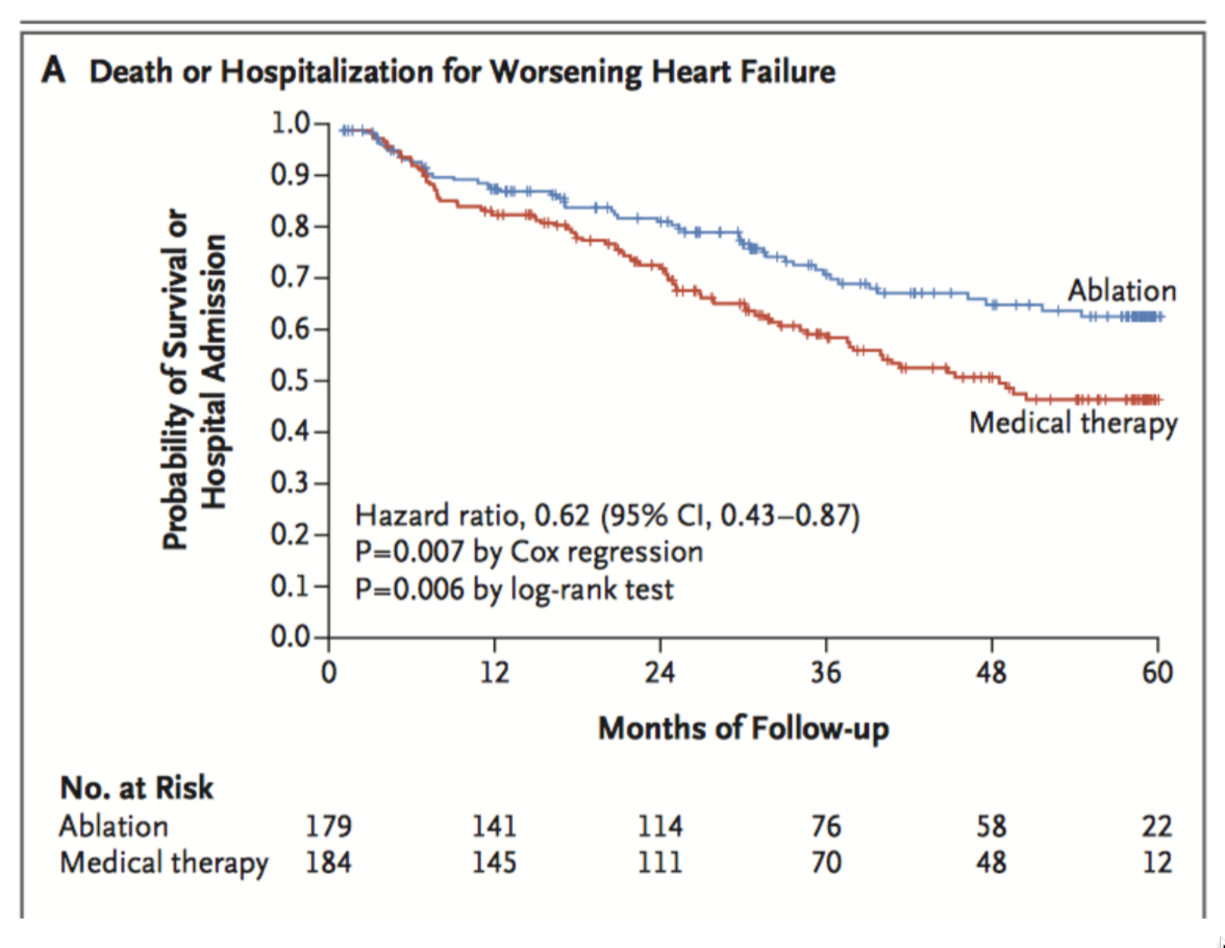
\includegraphics[width=0.7\textwidth,height=\textheight]{../figures/atrial_fib_death_hosp.pdf}
\caption{Figure from Marrouche, et al., \emph{NEJM} 2018}
\end{figure}

\end{frame}

\begin{frame}{%
\protect\hypertarget{example-clinical-trial-pbt01}{%
Example: Clinical trial PBT01}}

\begin{figure}
\centering
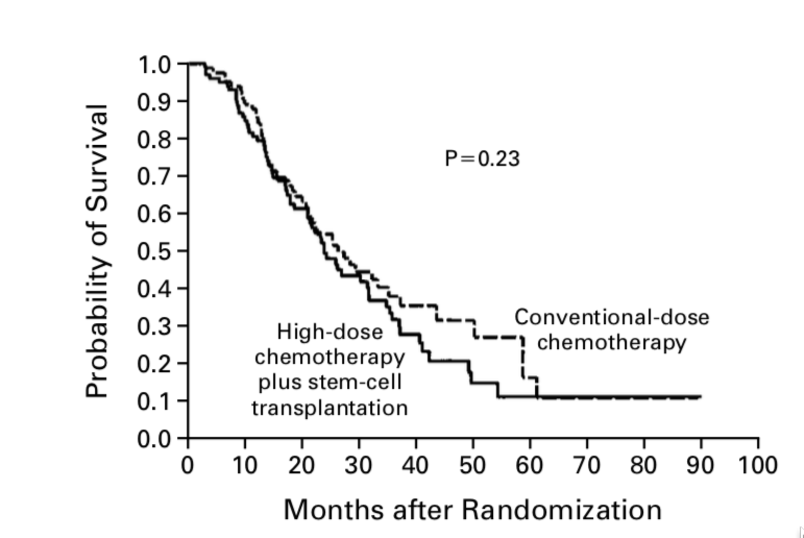
\includegraphics[width=0.7\textwidth,height=\textheight]{../figures/pbt01_survival.pdf}
\caption{Figure from Stadtmauer, et al, NEJM 2000}
\end{figure}

The next slides reproduce this figure and \(p\)-value from patient-level
data.

\end{frame}

\begin{frame}[fragile]{%
\protect\hypertarget{numerical-summary}{%
Numerical summary}}

\scriptsize

\begin{Shaded}
\begin{Highlighting}[]
\KeywordTok{library}\NormalTok{(survival)}
\KeywordTok{library}\NormalTok{(eventtimedata)}
\KeywordTok{data}\NormalTok{(}\StringTok{"pbt01"}\NormalTok{)}

\NormalTok{pbt01.survival <-}\StringTok{ }\KeywordTok{survfit}\NormalTok{(}\KeywordTok{Surv}\NormalTok{(survival, died) }\OperatorTok{~}\StringTok{ }\NormalTok{treatment, }
                              \DataTypeTok{data =}\NormalTok{ pbt01)}
\NormalTok{pbt01.survival}
\end{Highlighting}
\end{Shaded}

\end{frame}

\begin{frame}[fragile]{%
\protect\hypertarget{numerical-summary-1}{%
Numerical summary \ldots}}

\scriptsize

\begin{verbatim}
## Call: survfit(formula = Surv(survival, died) ~ treatment, data = pbt01)
## 
##                     n events median 0.95LCL 0.95UCL
## treatment=abmt    101     64   23.7    20.8    31.6
## treatment=control  83     50   26.2    21.2    43.5
\end{verbatim}

\end{frame}

\begin{frame}[fragile]{%
\protect\hypertarget{figure}{%
Figure}}

\scriptsize

\begin{Shaded}
\begin{Highlighting}[]
\KeywordTok{library}\NormalTok{(survival)}
\KeywordTok{library}\NormalTok{(eventtimedata)}
\KeywordTok{data}\NormalTok{(}\StringTok{"pbt01"}\NormalTok{)}

\NormalTok{pbt01.logrank.chisq =}\StringTok{ }\KeywordTok{survdiff}\NormalTok{(}\KeywordTok{Surv}\NormalTok{(survival, died) }\OperatorTok{~}\StringTok{ }\NormalTok{treatment, }
                                \DataTypeTok{data =}\NormalTok{ pbt01)}\OperatorTok{$}\NormalTok{chisq}
\NormalTok{pbt01.logrank.pvalue =}\StringTok{ }\KeywordTok{pchisq}\NormalTok{(pbt01.logrank.chisq, }\DecValTok{1}\NormalTok{,}
                              \DataTypeTok{lower.tail =} \OtherTok{FALSE}\NormalTok{)}

\KeywordTok{plot}\NormalTok{(pbt01.survival, }\DataTypeTok{lty =} \DecValTok{2}\OperatorTok{:}\DecValTok{3}\NormalTok{, }\DataTypeTok{col =} \DecValTok{3}\OperatorTok{:}\DecValTok{4}\NormalTok{, }\DataTypeTok{mark.time =} \OtherTok{TRUE}\NormalTok{, }
     \DataTypeTok{xlab =} \StringTok{"Months after Randomization"}\NormalTok{, }
     \DataTypeTok{ylab =} \StringTok{"Probability of Survival"}\NormalTok{,}
     \DataTypeTok{axes =} \OtherTok{FALSE}\NormalTok{,}
     \DataTypeTok{cex =} \FloatTok{0.6}\NormalTok{)}
\KeywordTok{legend}\NormalTok{(}\DecValTok{40}\NormalTok{, }\FloatTok{1.0}\NormalTok{, }\KeywordTok{c}\NormalTok{(}\StringTok{"ABMT"}\NormalTok{, }\StringTok{"Control"}\NormalTok{), }\DataTypeTok{lty =} \DecValTok{2}\OperatorTok{:}\DecValTok{3}\NormalTok{, }\DataTypeTok{col =} \DecValTok{3}\OperatorTok{:}\DecValTok{4}\NormalTok{,}
       \DataTypeTok{cex =} \FloatTok{0.6}\NormalTok{)}
\KeywordTok{text}\NormalTok{(}\DecValTok{40}\NormalTok{, }\FloatTok{0.6}\NormalTok{, }\StringTok{"log-rank p-value = "}\NormalTok{, }\DataTypeTok{cex =} \FloatTok{0.6}\NormalTok{)}
\KeywordTok{text}\NormalTok{(}\DecValTok{55}\NormalTok{, }\FloatTok{.6}\NormalTok{, }\KeywordTok{round}\NormalTok{(pbt01.logrank.pvalue, }\DataTypeTok{digits =} \DecValTok{2}\NormalTok{), }\DataTypeTok{cex =} \FloatTok{0.6}\NormalTok{)}
\KeywordTok{text}\NormalTok{(}\DecValTok{70}\NormalTok{, }\FloatTok{0.6}\NormalTok{, }\StringTok{"(unstratified)"}\NormalTok{, }\DataTypeTok{cex =} \FloatTok{0.6}\NormalTok{)}
\KeywordTok{axis}\NormalTok{(}\DecValTok{1}\NormalTok{)}
\KeywordTok{axis}\NormalTok{(}\DecValTok{2}\NormalTok{)}
\end{Highlighting}
\end{Shaded}

\end{frame}

\begin{frame}

\scriptsize

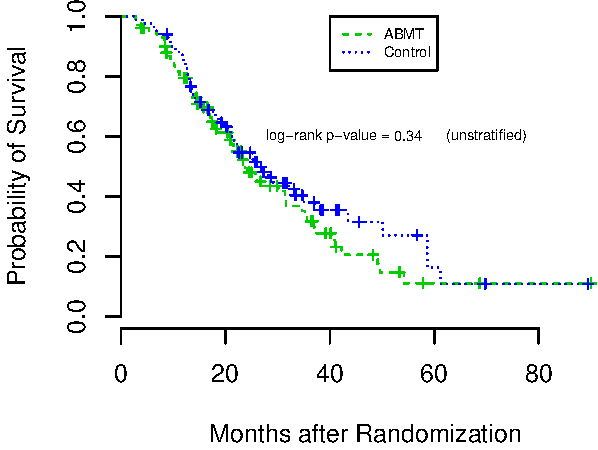
\includegraphics{unit_03_significance_testing_files/figure-beamer/unnamed-chunk-4-1.pdf}

\footnotesize

Note: The \(p\)-value is not identical to the one in the paper because
the paper used a stratified test, stratifying on the cycle needed to
induce complete response for the patient. Stratified tests coming later.

\end{frame}

\begin{frame}{%
\protect\hypertarget{parametric-vs-non-parametric-approaches}{%
Parametric vs non-parametric approaches}}

In the medical literature, survival analysis is often used in the study
of treatments for chronic diseases such as cancer, diabetes, or
cardiovascular disease.

In most studies, a proportion of participants have not had an event by
the time the study is analyzed.

\begin{itemize}
\tightlist
\item
  Thus, the right tail of the survival distribution is not observable.
\end{itemize}

Parametric approaches can be useful in some settings, but they assume a
model for the entire curve, and extrapolate tail behavior.

Non-parametric methods make no assumptions about tail behavior and are
less sensitive to outliers.

This section emphasizes \emph{non-parametric methods}.

\end{frame}

\begin{frame}{%
\protect\hypertarget{two-sample-non-parametric-tests-for-comparing-survival-distributions}{%
Two-sample non-parametric tests for comparing survival distributions}}

Comparing two distributions at a single time point

The log-rank test

Generalized Wilcoxon tests

The Fleming-Harrington family

\vspace{1cm}

\small

References:

\begin{tabular}{ll}
Hosmer \& Lemeshow &  Section 2.4\\
Collett & Section 2.5\\
Klein \& Moeschberger~~~~ & Section 7.3\\
\end{tabular}

\end{frame}

\hypertarget{comparing-two-distributions-at-a-single-time-point}{%
\section{Comparing two distributions at a single time
point}\label{comparing-two-distributions-at-a-single-time-point}}

\begin{frame}{%
\protect\hypertarget{using-widehats_1t-and-widehats_2t}{%
Using \(\widehat{S_1}(t)\) and \(\widehat{S_2}(t)\)}}

Sometimes a specific time point, \(t^{\star},\) is of special interest.

\begin{itemize}
\tightlist
\item
  e.g., 5-year disease-free survival in cancer
\end{itemize}

Simple method:

\begin{itemize}
\item
  Use the independence and approximate normality of
  \(\widehat S_k(t^\star); k \in\{ 0,1 \}\).
\item
  Examine a confidence interval for the difference in estimated survival
  curves at \(t^{\star}\).
\item
  Reject \(H_0: S_1(t) = S_2(t)\) in favor of a two-sided alternative if
  the interval does not include 0.
\end{itemize}

\end{frame}

\begin{frame}{%
\protect\hypertarget{confidence-interval-for-the-difference-of-two-survival-curves}{%
Confidence interval for the difference of two survival curves}}

The 95\% confidence interval is \[
\left[ \left ( \widehat S_1(t^\star) - \widehat S_0(t^\star) \right )
\pm 1.96 \times \sqrt{ V_1(t^\star) + V_0 (t^\star) }\right],
\] where \(V_k(t^\star)\) is the estimated variance of
\(\widehat S_k(t^\star).\)

This method is rarely used because

\begin{itemize}
\item
  it is not clear what \(t^\star\) should be
\item
  there is potential for abuse when applied \emph{post-hoc}
\end{itemize}

\end{frame}

\begin{frame}{%
\protect\hypertarget{example}{%
Example}}

Use numerical estimates of the survival curves to find a 95\% confidence
interval for the difference in survival curves at time point
\(t^\star = 10\) weeks for the Cox and Oakes leukemia data.

The following slides show the estimates repeated from Unit 2
(Estimation).

\end{frame}

\begin{frame}[fragile]{%
\protect\hypertarget{km-numerical-estimates-group-0}{%
KM numerical estimates, group == 0}}

\scriptsize

\begin{Shaded}
\begin{Highlighting}[]
\KeywordTok{library}\NormalTok{(survival)}
\KeywordTok{library}\NormalTok{(eventtimedata)}
\NormalTok{leukemia.group}\FloatTok{.0}\NormalTok{ =}\StringTok{ }
\StringTok{  }\KeywordTok{subset.data.frame}\NormalTok{(cox.oakes.leukemia, group }\OperatorTok{==}\StringTok{ }\DecValTok{0}\NormalTok{)}
\NormalTok{km.group}\FloatTok{.0}\NormalTok{ =}\StringTok{ }\KeywordTok{survfit}\NormalTok{(}\KeywordTok{Surv}\NormalTok{(time, relapse) }\OperatorTok{~}\StringTok{ }\DecValTok{1}\NormalTok{, }
                     \DataTypeTok{data =}\NormalTok{ leukemia.group}\FloatTok{.0}\NormalTok{)}
\KeywordTok{summary}\NormalTok{(km.group}\FloatTok{.0}\NormalTok{)}
\end{Highlighting}
\end{Shaded}

\begin{verbatim}
## Call: survfit(formula = Surv(time, relapse) ~ 1, data = leukemia.group.0)
## 
##  time n.risk n.event survival std.err lower 95% CI upper 95% CI
##     1     21       2   0.9048  0.0641      0.78754        1.000
##     2     19       2   0.8095  0.0857      0.65785        0.996
##     3     17       1   0.7619  0.0929      0.59988        0.968
##     4     16       2   0.6667  0.1029      0.49268        0.902
##     5     14       2   0.5714  0.1080      0.39455        0.828
##     8     12       4   0.3810  0.1060      0.22085        0.657
##    11      8       2   0.2857  0.0986      0.14529        0.562
##    12      6       2   0.1905  0.0857      0.07887        0.460
##    15      4       1   0.1429  0.0764      0.05011        0.407
##    17      3       1   0.0952  0.0641      0.02549        0.356
##    22      2       1   0.0476  0.0465      0.00703        0.322
##    23      1       1   0.0000     NaN           NA           NA
\end{verbatim}

\end{frame}

\begin{frame}[fragile]{%
\protect\hypertarget{km-numerical-estimates-group-1}{%
KM numerical estimates, group == 1}}

\scriptsize

\begin{Shaded}
\begin{Highlighting}[]
\NormalTok{leukemia.group}\FloatTok{.1}\NormalTok{ =}\StringTok{ }
\StringTok{  }\KeywordTok{subset.data.frame}\NormalTok{(cox.oakes.leukemia, group }\OperatorTok{==}\StringTok{ }\DecValTok{1}\NormalTok{)}
\NormalTok{km.group}\FloatTok{.1}\NormalTok{ =}\StringTok{ }\KeywordTok{survfit}\NormalTok{(}\KeywordTok{Surv}\NormalTok{(time, relapse) }\OperatorTok{~}\StringTok{ }\DecValTok{1}\NormalTok{, }
                     \DataTypeTok{data =}\NormalTok{ leukemia.group}\FloatTok{.1}\NormalTok{)}
\KeywordTok{summary}\NormalTok{(km.group}\FloatTok{.1}\NormalTok{)}
\end{Highlighting}
\end{Shaded}

\begin{verbatim}
## Call: survfit(formula = Surv(time, relapse) ~ 1, data = leukemia.group.1)
## 
##  time n.risk n.event survival std.err lower 95% CI upper 95% CI
##     6     21       3    0.857  0.0764        0.720        1.000
##     7     17       1    0.807  0.0869        0.653        0.996
##    10     15       1    0.753  0.0963        0.586        0.968
##    13     12       1    0.690  0.1068        0.510        0.935
##    16     11       1    0.627  0.1141        0.439        0.896
##    22      7       1    0.538  0.1282        0.337        0.858
##    23      6       1    0.448  0.1346        0.249        0.807
\end{verbatim}

\normalsize

\end{frame}

\begin{frame}{%
\protect\hypertarget{calculations}{%
Calculations \ldots}}

Lab exercise!

\end{frame}

\hypertarget{the-log-rank-test}{%
\section{The log-rank test}\label{the-log-rank-test}}

\begin{frame}{%
\protect\hypertarget{mantel-haenszel-log-rank-test}{%
Mantel-Haenszel log-rank test}}

The log-rank test is the most widely used non-parametric test.

Begin with a \(2 \times 2\) table classifying those with and without the
event of interest in a two group setting:

\begin{center}
\begin{tabular}{cccc}
\hline \hline
& \multicolumn{2}{c}{Event} & \\ \cline{2-3}
\multicolumn{1}{c}{Group } & ~~~~Yes~~~~ & ~~~~No~~~~ & ~~~Total~~~\\ \hline
0 & $d_0$ & $n_0 - d_0$ & $n_0$  \\
1 & $d_1$ & $n_1 - d_1$ & $n_1$ \\
\hline
Total &  $d  $ & $n   - d  $ & $n  $  \\ \hline \hline
\end{tabular}
\end{center}

The table shows the observed numbers with and without events in each
group, and the margin totals.

\end{frame}

\begin{frame}{%
\protect\hypertarget{mantel-haenszel-approach-to-a-2times2-table}{%
Mantel-Haenszel approach to a \(2\times2\) table}}

Define \(D_0\) as the random variable representing the number with an
event in Group 0.

If the margins of this table \((d, n-d, n_0, n_1)\) are considered
fixed, then \(D_0\) follows a hypergeometric distribution, depending on
one parameter (the population odds ratio, \(\psi\)).

Under \(H_0\), the null hypothesis of no association between the event
and group:
\[E(D_0) = \frac{n_0 \, d}{n} = n_0 \left(\frac{d}{n}\right) \]

\[\text{Var}(D_0) = \frac{n_0 \, n_1 \, d(n-d)}{n^2 (n-1)} \]

\end{frame}

\begin{frame}{%
\protect\hypertarget{mantel-haenszel-approach-to-a-2times2-table-1}{%
Mantel-Haenszel approach to a \(2\times2\) table\ldots}}

Thus, the Mantel-Haenszel statistic is
\[\chi^2_{\tiny MH } = \frac{\left[d_0-n_0 \, d/n\right]^2}{\frac{n_0
\, n_1 \, d(n-d)} {n^2 (n-1)}} \sim \chi^2_1
\]

\(\chi^2_{\tiny MH}\) is approximately equivalent to the Pearson
\(\chi^2\) test for equality of the two groups given by:
\[\chi^2_p = \sum \frac{(o-e)^2}{e}, \] where \(o\) represents observed
values and \(e\) the expected values.

\end{frame}

\begin{frame}{%
\protect\hypertarget{example-toxicity-in-a-clinical-trial-with-two-treatments}{%
Example: Toxicity in a clinical trial with two treatments}}

\begin{center}
\begin{tabular}{cccc}
\hline \hline
& \multicolumn{2}{c}{Toxicity}   \\ \cline{2-3}
\multicolumn{1}{c}{Group } & ~~~Yes~~~ & ~~~No~~~ & ~~~Total~~~ \\ \hline
0 &  ~8    & 42  &  ~50       \\
1 &  ~2   &  48 &   ~50        \\
\hline
Total & 10 & 90 &  100        \\ \hline \hline
\end{tabular}
\end{center}

\begin{align*}
\chi_p^2 &= 4.00 ~~~~ (p=0.046)\\[3ex]
\chi_{\tiny MH}^2 &= 3.96 ~~~~ (p=0.047)
\end{align*}

\end{frame}

\begin{frame}{%
\protect\hypertarget{pearson-chi2-vs-mh}{%
Pearson \(\chi^2\) vs MH}}

\emph{Note:} the Pearson \(\chi^2\) test applies to the case where the
row margins are fixed but not the column margins, as a test of
equivalence between the proportions with events in the two groups.

In this case, the variance is slightly different: \[
\text{Var}(D_0) = \frac{n_0 \, n_1 \, d(n-d)}{n^3}
\]

\end{frame}

\begin{frame}{%
\protect\hypertarget{for-the-case-of-k-tables}{%
For the case of \(K\) tables}}

Now suppose there are \(K\) \(2 \times 2\) tables, all independent.

The goal is to test for a common group effect \(H_0: \psi_j=\psi=1\)
versus \(H_A: \psi \neq 1\).

The \emph{Cochran-Mantel-Haenszel test} for a common odds ratio not
equal to 1 can be written as:

\[  
\chi^2_{CMH} =   \frac{\left[ {\sum_{j=1}^K (d_{0j} - n_{0j} \times d_j/n_j)}\right]^2}
        {\sum_{j=1}^K n_{1j} n_{0j} d_j (n_j-d_j)/[n_j^2(n_j-1)]}  \]

This statistic is distributed approximately as \(\chi^2_1\).

\end{frame}

\begin{frame}{%
\protect\hypertarget{k-tables}{%
\(K\) tables \ldots}}

The subscript \(j\) refers to the \(j\)-th table:

\begin{center}
\begin{tabular}{cccc}
\hline \hline
& \multicolumn{2}{c}{Event} & \\ \cline{2-3}
\multicolumn{1}{c}{Group } & ~~~Yes~~~ & ~~~No~~~ & ~~~Total~~~\\ \hline
0 & $d_{0j}$ & $n_{0j} - d_{0j}$ & $n_{0j}$  \\
1 & $d_{1j}$ & $n_{1j} - d_{1j}$ & $n_{1j}$ \\
\hline
Total &  $d_j  $ & $n_j - d_j  $ & $n_j  $  \\ \hline \hline
\end{tabular}
\end{center}

\end{frame}

\begin{frame}{%
\protect\hypertarget{log-rank-test-applying-cmh-to-survival-data}{%
Log-rank Test: Applying CMH to survival data}}

For the two-group \emph{log-rank} test:

\begin{itemize}
\item
  Construct a \(2 \times 2\) table at each distinct failure time.
\item
  Compare the failure rates between the two groups, conditional on the
  number at risk in the groups.
\item
  Combine the results from each table using the Cochran-Mantel-Haenszel
  test.
\end{itemize}

\end{frame}

\begin{frame}{%
\protect\hypertarget{formal-notation-for-the-log-rank-test}{%
Formal notation for the log-rank test}}

Let \(t_1, \ldots ,t_K\) represent the \(K\) ordered, distinct failure
times.

The table at the \(j\)-th failure time, is

\begin{center}
\begin{tabular}{cccc}
\hline \hline
& \multicolumn{2}{c}{Die/Fail} & \\ \cline{2-3}
\multicolumn{1}{c}{Group } & ~~~Yes~~~ & ~~~No~~~ & ~~Total~~\\ \hline
0 & $d_{0j}$ & $r_{0j} - d_{0j}$ & $r_{0j}$ \\[2ex]
1 & $d_{1j}$ & $r_{1j} - d_{1j}$ & $r_{1j}$ \\[2ex]
\hline
Total &  $d_j$ & $r_j - d_j$ & $r_j$  \\ \hline \hline
\end{tabular}
\end{center}

where

\begin{itemize}
\item
  \(d_{0j}\) and \(d_{1j}\) are the number of failures in group 0 and 1,
  respectively, at the \(j\)-th failure time
\item
  \(r_{0j}\) and \(r_{1j}\) are the number at risk in groups 0 and 1, at
  the \(j\)-th failure time
\end{itemize}

\end{frame}

\begin{frame}{%
\protect\hypertarget{the-log-rank-test-statistic-formula}{%
The log-rank test statistic formula}}

\begin{align*}
\chi^2_{\text{log-rank}} &=
\frac{\left[{\sum_{j=1}^K (d_{0j} - r_{0j} \times d_j/r_j)}\right]^2}
{\sum_{j=1}^K  \frac{r_{1j} r_{0j} d_j (r_j-d_j)}{[r_j^2(r_j-1)]}}
\end{align*}

If the tables are all independent, then this statistic will have an
approximate \(\chi^2\) distribution with 1 df.

\end{frame}

\begin{frame}{%
\protect\hypertarget{notes-about-log-rank-tests}{%
Notes about log-rank tests}}

The log-rank statistic depends on ranks of event times only, that is, on
the order in which events and censorings occur.

If there are no tied failure times between the two groups, then
\(d_j=1\) and the log-rank statistic simplifies to
\[\chi^2_{\text{log-rank}}  =  \frac{[\sum_{j=1}^K (d_{0j} - \frac{r_{0j}}{r_j})]^2}
        {\sum_{j=1}^K r_{1j}r_{0j}/r_j^2}  \]

The numerator can be interpreted as \([\sum (o-e)]^2\), where

\begin{itemize}
\item
  \(o\) is the observed number of deaths in a group, and \(e\) is the
  expected number, given the risk sets.
\item
  The expected number equals the number of failures times the proportion
  at risk in the group.
\item
  It does not matter which group is used for the sum.
\end{itemize}

\end{frame}

\begin{frame}{%
\protect\hypertarget{notes-about-the-log-rank}{%
Notes about the log-rank\ldots}}

The (\(o-e\)) terms in the numerator can be written as
\[   \frac{r_{0j}r_{1j}}{r_j}(\widehat\lambda_{1j} - \widehat\lambda_{0j} ) \]

Solution as a lab problem!

\end{frame}

\begin{frame}{%
\protect\hypertarget{assumptions-behind-log-rank-test}{%
Assumptions behind log-rank test}}

Censoring is independent.

\begin{itemize}
\tightlist
\item
  This assumption is made in nearly all survival methods.
\end{itemize}

The contributions to the statistic made by the \(2 \times 2\) tables can
be treated as independent.

\begin{itemize}
\tightlist
\item
  Proven true in the 1980’s
\end{itemize}

The log-rank test is most powerful when hazards have a constant ratio
over time.

\begin{itemize}
\item
  This is termed the \emph{proportional hazards} assumption.
\item
  It is not required for validity under the null hypothesis.
\end{itemize}

\end{frame}

\begin{frame}{%
\protect\hypertarget{efficiency-of-the-log-rank-test}{%
Efficiency of the log-rank test}}

The CMH test for a series of tables stratified by a potential confounder
is most powerful when \ldots  

\begin{itemize}
\tightlist
\item
  The tables have a constant odds ratio.
\end{itemize}

Analogously, the log-rank test is most powerful when \ldots

\begin{itemize}
\item
  The hazard ratios are constant across \(t\) time intervals.
\item
  This corresponds to \emph{proportional hazards}.
\end{itemize}

\end{frame}

\begin{frame}{%
\protect\hypertarget{the-recidivism-data}{%
The recidivism data}}

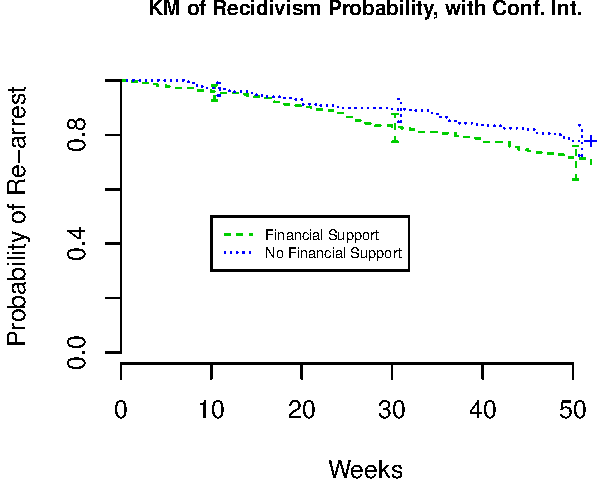
\includegraphics{unit_03_significance_testing_files/figure-beamer/unnamed-chunk-7-1.pdf}

\end{frame}

\begin{frame}[fragile]{%
\protect\hypertarget{the-recidivism-data-1}{%
The recidivism data \ldots}}

\scriptsize

\begin{Shaded}
\begin{Highlighting}[]
\KeywordTok{library}\NormalTok{(survival)}
\KeywordTok{library}\NormalTok{(eventtimedata)}
\KeywordTok{data}\NormalTok{(}\StringTok{"rossi"}\NormalTok{)}
\KeywordTok{survfit}\NormalTok{(}\KeywordTok{Surv}\NormalTok{(week, arrest) }\OperatorTok{~}\StringTok{ }\NormalTok{fin, }
                        \DataTypeTok{data =}\NormalTok{ rossi)}
\end{Highlighting}
\end{Shaded}

\begin{verbatim}
## Call: survfit(formula = Surv(week, arrest) ~ fin, data = rossi)
## 
##           n events median 0.95LCL 0.95UCL
## fin=no  216     66     NA      NA      NA
## fin=yes 216     48     NA      NA      NA
\end{verbatim}

\begin{Shaded}
\begin{Highlighting}[]
\KeywordTok{survdiff}\NormalTok{(}\KeywordTok{Surv}\NormalTok{(week, arrest) }\OperatorTok{~}\StringTok{ }\NormalTok{fin, }
                        \DataTypeTok{data =}\NormalTok{ rossi)}
\end{Highlighting}
\end{Shaded}

\begin{verbatim}
## Call:
## survdiff(formula = Surv(week, arrest) ~ fin, data = rossi)
## 
##           N Observed Expected (O-E)^2/E (O-E)^2/V
## fin=no  216       66     55.6      1.96      3.84
## fin=yes 216       48     58.4      1.86      3.84
## 
##  Chisq= 3.8  on 1 degrees of freedom, p= 0.0501
\end{verbatim}

\end{frame}

\begin{frame}{%
\protect\hypertarget{what-does-non-proportional-hazards-look-like}{%
What does non-proportional hazards look like?}}

The next slides show figures presented at a February 5, 2018 meeting on
non-proportional hazards.

All use data from published papers.

The workshop (sponsored by Duke University Margolis Center)

\begin{itemize}
\item
  reviewed instances where non-proportional hazards occurred in studies
  designed for drug approval
\item
  discussed strategies for modifying usual methods of analysis
\end{itemize}

\end{frame}

\begin{frame}{%
\protect\hypertarget{randomized-trial-in-prostate-cancer}{%
Randomized trial in prostate cancer}}

\begin{figure}
\centering
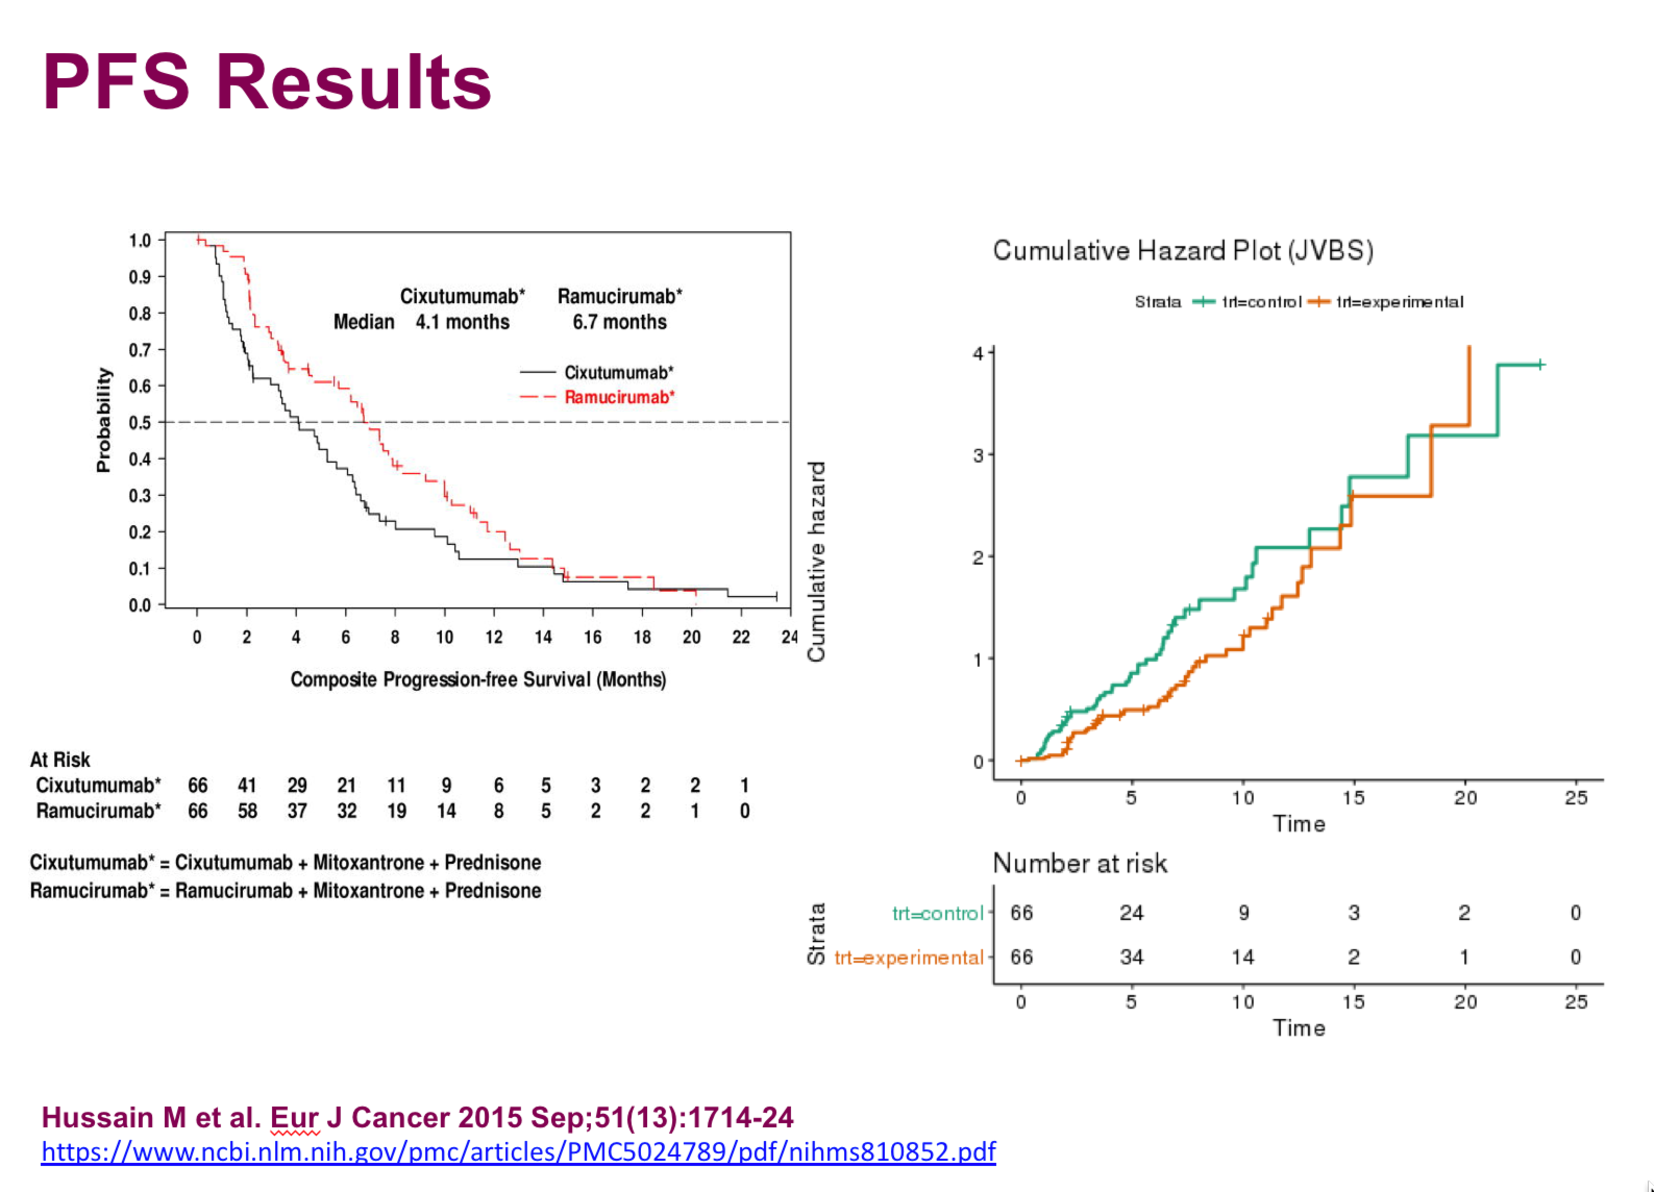
\includegraphics[width=0.8\textwidth,height=\textheight]{../figures/hussain.pdf}
\caption{Data from Hussain, et al., \emph{Euro J Cancer}, 2015}
\end{figure}

See \href{../../clinical_papers/hussain.pdf}{Hussain, et al.}

\end{frame}

\begin{frame}{%
\protect\hypertarget{rct-in-acute-leukemia}{%
RCT in acute leukemia}}

\begin{figure}
\centering

\includegraphics[width=0.8\textwidth,height=\textheight]{../figures/kantarjian.pdf}
\caption{KM survival curves from Kantarjian, et al., \emph{NEJM}, 2016}
\end{figure}

See \href{../../kantarjian.pdf}{Kantarjian, et al.}

\end{frame}

\begin{frame}{%
\protect\hypertarget{rct-in-acute-leukemia-1}{%
RCT in acute leukemia \ldots}}

\begin{figure}
\centering
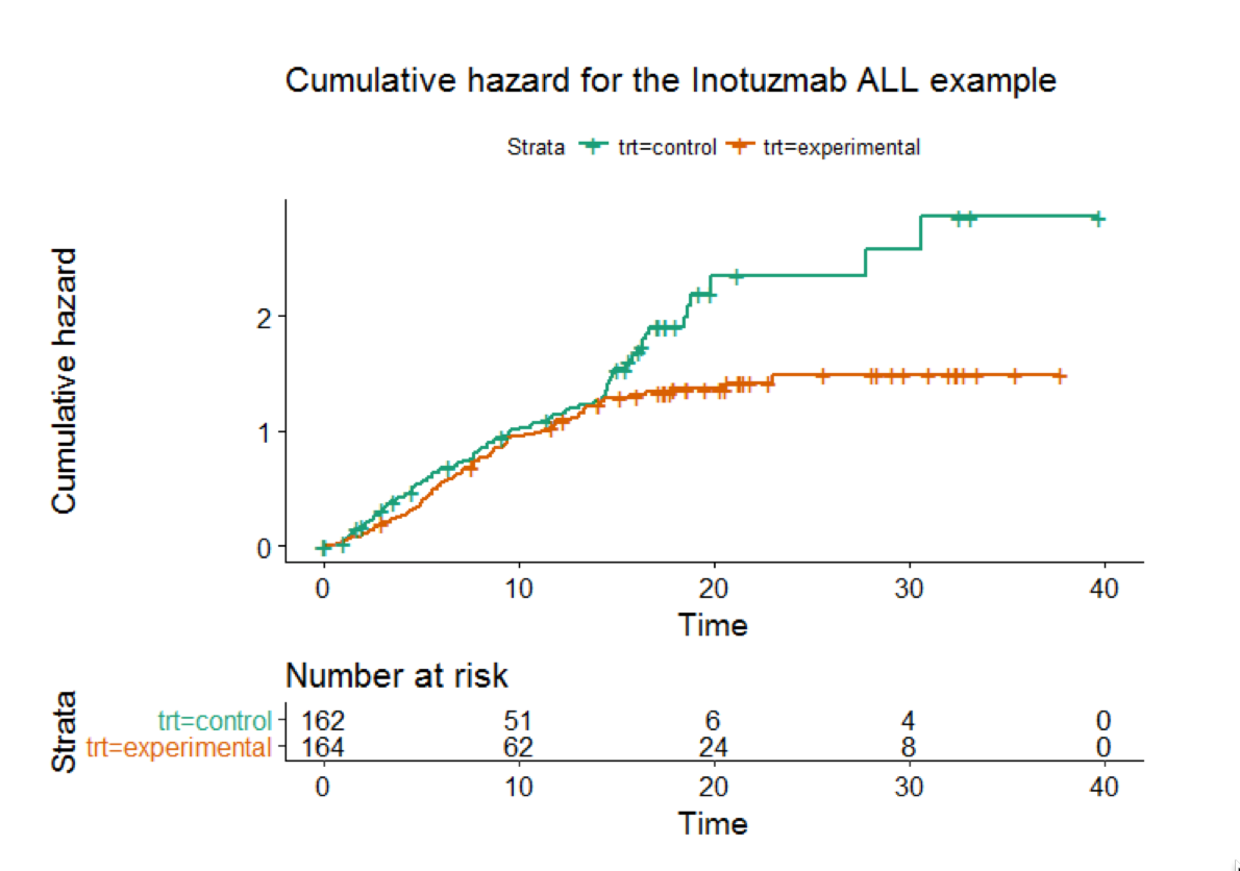
\includegraphics[width=0.8\textwidth,height=\textheight]{../figures/cum_haz_ALL.pdf}
\caption{Cumulative hazards from Kantarjian, et al., \emph{NEJM}, 2016}
\end{figure}

\end{frame}

\begin{frame}[fragile]{%
\protect\hypertarget{another-example-but-with-data}{%
Another example, but with data}}

\scriptsize

\begin{Shaded}
\begin{Highlighting}[]
\CommentTok{#library(devtools)}
\CommentTok{#install_github("keaven/nphsim")}
\KeywordTok{library}\NormalTok{(survival)}
\KeywordTok{library}\NormalTok{(nphsim)}
\KeywordTok{data}\NormalTok{(Ex6crossing)}
\KeywordTok{survfit}\NormalTok{(}\KeywordTok{Surv}\NormalTok{(month,evntd) }\OperatorTok{~}\StringTok{ }\NormalTok{trt, }\DataTypeTok{data =}\NormalTok{ Ex6crossing)}
\end{Highlighting}
\end{Shaded}

\begin{verbatim}
## Call: survfit(formula = Surv(month, evntd) ~ trt, data = Ex6crossing)
## 
##         n events median 0.95LCL 0.95UCL
## trt=0 145    111  10.66    8.83    12.5
## trt=1 145    113   9.92    7.38    14.3
\end{verbatim}

\begin{Shaded}
\begin{Highlighting}[]
\KeywordTok{survdiff}\NormalTok{(}\KeywordTok{Surv}\NormalTok{(month,evntd) }\OperatorTok{~}\StringTok{ }\NormalTok{trt, }\DataTypeTok{data =}\NormalTok{ Ex6crossing)}
\end{Highlighting}
\end{Shaded}

\begin{verbatim}
## Call:
## survdiff(formula = Surv(month, evntd) ~ trt, data = Ex6crossing)
## 
##         N Observed Expected (O-E)^2/E (O-E)^2/V
## trt=0 145      111      110    0.0147    0.0296
## trt=1 145      113      114    0.0141    0.0296
## 
##  Chisq= 0  on 1 degrees of freedom, p= 0.863
\end{verbatim}

\end{frame}

\begin{frame}{%
\protect\hypertarget{the-kaplan-meier-estimate}{%
The Kaplan-Meier estimate}}

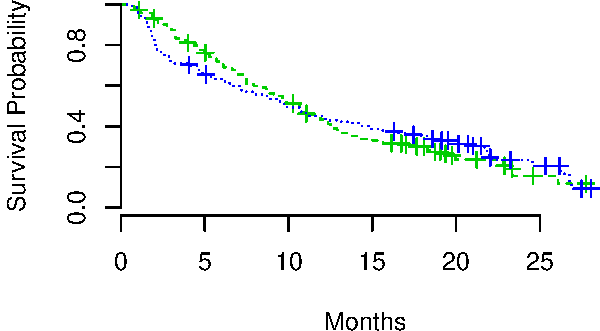
\includegraphics{unit_03_significance_testing_files/figure-beamer/unnamed-chunk-10-1.pdf}

\end{frame}

\begin{frame}{%
\protect\hypertarget{the-cumulative-hazard}{%
The cumulative hazard}}

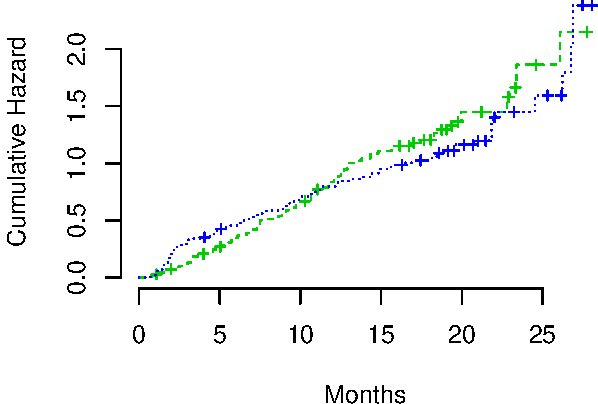
\includegraphics{unit_03_significance_testing_files/figure-beamer/unnamed-chunk-11-1.pdf}

\end{frame}

\hypertarget{weighted-log-rank-tests}{%
\section{Weighted log-rank tests}\label{weighted-log-rank-tests}}

\begin{frame}{%
\protect\hypertarget{the-tarone-ware-class-of-tests}{%
The Tarone-Ware class of tests}}

\small

This general class of tests is like the log-rank test, but adds weights
\({w_j}\).

Many specific test statistics are included as special cases.
\[ \chi^2_{TW} = \frac{[\sum_{j=1}^K {w_j} (d_{1j} - r_{1j} \times d_j/r_j)]^2}
        {\sum_{l=1}^K \frac{w_j^2 r_{1j}r_{0j}d_j(r_j-d_j)}{r_j^2(r_j-1)}}  \]

\begin{center}
\begin{tabular}{ll}
\hline \hline
Test statistic &  Weight ${w_j}$ \\ \hline
Log-rank              &  $w_j = 1$\\[2ex]
Gehan's Wilcoxon     &  $w_j = r_j$\\[2ex]
Peto/Prentice Wilcoxon       &  $w_j = n \widehat{S}(t_j)$\\[2ex]
Fleming-Harrington~~~~   &  $w_j=[\widehat{S}(t_j)]^\rho ~ [1-\widehat{S}(t_j)]^\gamma$\\[2ex]
Tarone-Ware          &  $w_j=\sqrt{r_j}$\\
\hline \hline
\end{tabular}
\end{center}

\(r_j\) is the number of subjects at risk at the \(j^{th}\) event time.

\end{frame}

\begin{frame}{%
\protect\hypertarget{some-background}{%
Some background}}

The generalized Wilcoxon tests precede the Tarone-Ware or
Fleming-Harrington class of tests.

\begin{itemize}
\item
  The Gehan-Wilcoxon was derived using a generalization of the \(U\)
  statistic approach to the Mann-Whitney-Wilcoxon.
\item
  The Peto/Prentice Wilcoxon was derived using a generalization of
  linear rank statistics.
\end{itemize}

\end{frame}

\begin{frame}{%
\protect\hypertarget{more-details-on-the-fleming-harrington-test}{%
More details on the Fleming-Harrington test}}

The parameters \(\rho\) and \(\gamma\) can be any non-negative numbers:

\begin{itemize}
\item
  If \(\rho = \gamma = 0\), \(w_j=1\) and the test is the usual log-rank
  test.
\item
  If \(\rho=1\) and \(\gamma=0\), the test is similar to the
  Peto-Prentice.\footnote{This is the default ``Fleming'' test in SAS PROC LIFETEST.}
\item
  If \(\rho=0\) and \(\gamma=1\), what happens to \(w_j\) over follow-up
  time?
\item
  If \(\rho = \gamma = 1\), the weight \(w_j\) reaches a maximum at the
  median, and is smaller for both large and small \(t_j\).
\end{itemize}

The \texttt{survdiff()} function in \textsf{R} sets \(\gamma=0\) and
allows the user to set \(\rho\).

\end{frame}

\begin{frame}[fragile]{%
\protect\hypertarget{earlier-numerical-example-rho-1}{%
Earlier numerical example, \(\rho = 1\)}}

\small

This is a generalized Wilcoxon test

\begin{Shaded}
\begin{Highlighting}[]
\CommentTok{#library(devtools)}
\CommentTok{#install_github("keaven/nphsim")}
\KeywordTok{library}\NormalTok{(survival)}
\KeywordTok{library}\NormalTok{(nphsim)}
\KeywordTok{data}\NormalTok{(Ex6crossing)}
\KeywordTok{survdiff}\NormalTok{(}\KeywordTok{Surv}\NormalTok{(month,evntd) }\OperatorTok{~}\StringTok{ }\NormalTok{trt, }\DataTypeTok{rho =} \DecValTok{1}\NormalTok{, }\DataTypeTok{data =}\NormalTok{ Ex6crossing)}
\end{Highlighting}
\end{Shaded}

\begin{verbatim}
## Call:
## survdiff(formula = Surv(month, evntd) ~ trt, data = Ex6crossing, 
##     rho = 1)
## 
##         N Observed Expected (O-E)^2/E (O-E)^2/V
## trt=0 145     65.7     69.1     0.173     0.509
## trt=1 145     70.5     67.1     0.178     0.509
## 
##  Chisq= 0.5  on 1 degrees of freedom, p= 0.476
\end{verbatim}

\end{frame}

\begin{frame}[fragile]{%
\protect\hypertarget{earlier-numerical-example-rho-2}{%
Earlier numerical example, \(\rho = 2\)}}

\small

\begin{Shaded}
\begin{Highlighting}[]
\CommentTok{#library(devtools)}
\CommentTok{#install_github("keaven/nphsim")}
\KeywordTok{library}\NormalTok{(survival)}
\KeywordTok{library}\NormalTok{(nphsim)}
\KeywordTok{data}\NormalTok{(Ex6crossing)}
\KeywordTok{survdiff}\NormalTok{(}\KeywordTok{Surv}\NormalTok{(month,evntd) }\OperatorTok{~}\StringTok{ }\NormalTok{trt, }\DataTypeTok{rho =} \DecValTok{2}\NormalTok{, }\DataTypeTok{data =}\NormalTok{ Ex6crossing)}
\end{Highlighting}
\end{Shaded}

\begin{verbatim}
## Call:
## survdiff(formula = Surv(month, evntd) ~ trt, data = Ex6crossing, 
##     rho = 2)
## 
##         N Observed Expected (O-E)^2/E (O-E)^2/V
## trt=0 145     43.6     49.2     0.637      2.15
## trt=1 145     51.8     46.2     0.679      2.15
## 
##  Chisq= 2.2  on 1 degrees of freedom, p= 0.142
\end{verbatim}

\end{frame}

\begin{frame}{%
\protect\hypertarget{be-careful-with-weighted-lr-tests}{%
Be careful with weighted LR tests}}

The weighted LR tests are often presented as emphasizing differences
between two hazard functions.

For the F-H weights,
\((\widehat{S}(t))^\rho(1 - \widehat{S}(t))^\gamma\),

\begin{itemize}
\item
  \(\rho > 0,\,\, \gamma = 0\): weights early differences (\(\rho = 1\)
  gen Wilcoxon)
\item
  \(\rho = 0,\,\, \gamma > 0\): weights late differences
\item
  \(\rho > 0,\,\, \gamma > 0\): weights differences near median
\item
  \(\rho = 0,\,\, \gamma = 0\): weights differences equally over time
  (log-rank)
\end{itemize}

Choosing the test post-hoc, based on observed data, leads to potentially
increased Type I error.

The
\href{https://healthpolicy.duke.edu/events/public-workshop-oncology-clinical-trials-presence-non-proportional-hazards}{February
2018 Duke-Margolis workshop} discussed ways to specify these tests in
design and sample size calculations.

\begin{itemize}
\tightlist
\item
  Full workshop materials available at the link.
\end{itemize}

\end{frame}

\hypertarget{tests-for-more-than-two-groups}{%
\section{Tests for more than two
groups}\label{tests-for-more-than-two-groups}}

\begin{frame}{%
\protect\hypertarget{introduction-1}{%
Introduction}}

Suppose data come from \(P\) different groups. The data from group \(p\)
(\(p=1,\ldots,P\)) are: \[ (X_{p1},\delta_{p1}) \dots
(X_{p n_p},\delta_{p n_p}) \]

Tests are based on a \(P \times 2\) table at each distinct \(K\) failure
time.

\begin{itemize}
\item
  Compare the event rates between the \(P\) groups, conditional on the
  number at risk, combining the tables using the CMH approach
\item
  Final test statistic has \(\chi^2\) distribution with \(P - 1\)
  degrees of freedom
\end{itemize}

\end{frame}

\begin{frame}{%
\protect\hypertarget{example-prognosis-in-lymphoma}{%
Example: prognosis in lymphoma}}

The data \texttt{lymphoma.prognosis} in the package
\texttt{eventtimedata} was used as the training sample in the
International Prognostic Index published by
\href{../../clinical_papers/shipp_int_prog_index_nejm.pdf}{Shipp, et
al.} in 1993.

The data record survival time and censoring for 1,385 patients with
non-Hodgkin’s lymphoma treated at sites in the US, Canada, and Europe.

In this analysis, we look at the association of disease stage and
survival. See the package documentation for the variable definitions.

\end{frame}

\begin{frame}[fragile]{%
\protect\hypertarget{the-code-for-the-4-group-test}{%
The code for the 4-group test}}

\footnotesize

\begin{Shaded}
\begin{Highlighting}[]
\KeywordTok{library}\NormalTok{(survival)}
\KeywordTok{library}\NormalTok{(eventtimedata)}
\KeywordTok{data}\NormalTok{(lymphoma.prognosis)}

\NormalTok{stage.factor =}\StringTok{ }\KeywordTok{as.factor}\NormalTok{(lymphoma.prognosis}\OperatorTok{$}\NormalTok{STAGE)}
\NormalTok{died =}\StringTok{ }\NormalTok{lymphoma.prognosis}\OperatorTok{$}\NormalTok{SURVIVAL }\OperatorTok{-}\StringTok{ }\DecValTok{1}
\NormalTok{died[died }\OperatorTok{==}\StringTok{ }\DecValTok{2}\NormalTok{] =}\StringTok{ }\DecValTok{0}  \CommentTok{#recoding those lost to follow-up as censored}
\NormalTok{survival.time =}\StringTok{ }\NormalTok{lymphoma.prognosis}\OperatorTok{$}\NormalTok{SURVTIME}
\NormalTok{lymphoma.survival <-}\StringTok{ }\KeywordTok{survfit}\NormalTok{(}\KeywordTok{Surv}\NormalTok{(survival.time, died) }\OperatorTok{~}\StringTok{ }
\StringTok{                               }\NormalTok{stage.factor)}
\NormalTok{lymphoma.survival}
\KeywordTok{survdiff}\NormalTok{(}\KeywordTok{Surv}\NormalTok{(survival.time, died) }\OperatorTok{~}\StringTok{ }\NormalTok{stage.factor)}
\end{Highlighting}
\end{Shaded}

\end{frame}

\begin{frame}[fragile]{%
\protect\hypertarget{the-output-for-the-4-group-test}{%
The output for the 4-group test}}

\footnotesize

\begin{verbatim}
## Call: survfit(formula = Surv(survival.time, died) ~ stage.factor)
## 
##                  n events median 0.95LCL 0.95UCL
## stage.factor=1  93     24     NA    6.39      NA
## stage.factor=2 419    127     NA    7.30      NA
## stage.factor=3 253    112   5.70    4.11      NA
## stage.factor=4 620    340   2.68    1.84    4.22
\end{verbatim}

\begin{verbatim}
## Call:
## survdiff(formula = Surv(survival.time, died) ~ stage.factor)
## 
##                  N Observed Expected (O-E)^2/E (O-E)^2/V
## stage.factor=1  93       24     48.6   12.4446    13.559
## stage.factor=2 419      127    201.0   27.2575    41.012
## stage.factor=3 253      112    114.4    0.0502     0.062
## stage.factor=4 620      340    239.0   42.6908    71.011
## 
##  Chisq= 82.8  on 3 degrees of freedom, p= 0
\end{verbatim}

\end{frame}

\begin{frame}{%
\protect\hypertarget{the-survival-plot}{%
The survival plot}}

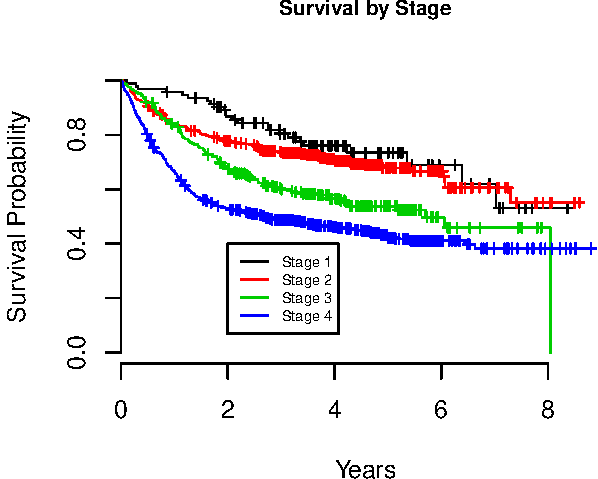
\includegraphics{unit_03_significance_testing_files/figure-beamer/unnamed-chunk-16-1.pdf}

\end{frame}

\hypertarget{the-stratified-log-rank-test}{%
\section{The stratified log-rank
test}\label{the-stratified-log-rank-test}}

\begin{frame}{%
\protect\hypertarget{example-length-of-stay-in-a-nursing-home}{%
Example: length of stay in a nursing home}}

The National Center for Health Services Research studied 36 for-profit
nursing homes to assess

\begin{itemize}
\tightlist
\item
  effects of different financial incentives on length of stay
\end{itemize}

``Treated" nursing homes received

\begin{itemize}
\item
  Higher daily reimbursements for US Medicaid (financially needy)
  patients
\item
  Bonuses for improving a patient’s health and sending them home
\end{itemize}

Study included 1601 patients admitted between May 1, 1981 and April 30,
1982.\footnote{Data are in \texttt{nursing.home} in the \texttt{eventtimedata} package.}

\end{frame}

\begin{frame}[fragile]{%
\protect\hypertarget{differences-in-length-of-stay-by-treatment}{%
Differences in length of stay by treatment}}

\footnotesize

\begin{Shaded}
\begin{Highlighting}[]
\KeywordTok{library}\NormalTok{(survival)}
\KeywordTok{library}\NormalTok{(eventtimedata)}
\KeywordTok{data}\NormalTok{(nursing.home)}
\KeywordTok{survdiff}\NormalTok{(}\KeywordTok{Surv}\NormalTok{(stay, cens) }\OperatorTok{~}\StringTok{ }\NormalTok{rx, }\DataTypeTok{data =}\NormalTok{ nursing.home)}
\end{Highlighting}
\end{Shaded}

\begin{verbatim}
## Call:
## survdiff(formula = Surv(stay, cens) ~ rx, data = nursing.home)
## 
##                   N Observed Expected (O-E)^2/E (O-E)^2/V
## rx=Control      889      684      677    0.0822     0.179
## rx=Intervention 712      595      602    0.0923     0.179
## 
##  Chisq= 0.2  on 1 degrees of freedom, p= 0.672
\end{verbatim}

\end{frame}

\begin{frame}{%
\protect\hypertarget{a-stratified-analysis}{%
A stratified analysis}}

Length of stay may also be associated with gender.

\begin{itemize}
\tightlist
\item
  Women tend to be healthier in the US.
\end{itemize}

A stratified test allows one to test for treatment differences,
adjusting for gender (without using a modeling approach).

\begin{itemize}
\item
  assumes the shape of the hazard may vary between men and women, but
  that the effect of the incentive would be the same
\item
  easy to do in almost any software
\end{itemize}

\end{frame}

\begin{frame}[fragile]{%
\protect\hypertarget{differences-in-length-of-stay-by-treatment-stratified-by-gender}{%
Differences in length of stay by treatment, stratified by gender}}

\footnotesize

\begin{Shaded}
\begin{Highlighting}[]
\KeywordTok{library}\NormalTok{(survival)}
\KeywordTok{library}\NormalTok{(eventtimedata)}
\KeywordTok{data}\NormalTok{(nursing.home)}
\KeywordTok{survdiff}\NormalTok{(}\KeywordTok{Surv}\NormalTok{(stay, cens) }\OperatorTok{~}\StringTok{ }\NormalTok{rx }\OperatorTok{+}\StringTok{ }\KeywordTok{strata}\NormalTok{(gender), }
         \DataTypeTok{data =}\NormalTok{ nursing.home)}
\end{Highlighting}
\end{Shaded}

\begin{verbatim}
## Call:
## survdiff(formula = Surv(stay, cens) ~ rx + strata(gender), data = nursing.home)
## 
##                   N Observed Expected (O-E)^2/E (O-E)^2/V
## rx=Control      889      684      679    0.0370    0.0812
## rx=Intervention 712      595      600    0.0418    0.0812
## 
##  Chisq= 0.1  on 1 degrees of freedom, p= 0.776
\end{verbatim}

\end{frame}

\begin{frame}[fragile]{%
\protect\hypertarget{the-stratified-test-for-the-pbt01-data}{%
The stratified test for the PBT01 data}}

Log-rank test stratified on \texttt{cycle.of.resp}.

This is the \(p\)-value in the Stadtmauer paper.

\begin{itemize}
\tightlist
\item
  Unstratified \(p\)-value (shown in earlier slides) is 0.34.
\end{itemize}

\scriptsize

\begin{Shaded}
\begin{Highlighting}[]
\KeywordTok{library}\NormalTok{(survival)}
\KeywordTok{library}\NormalTok{(eventtimedata)}
\KeywordTok{data}\NormalTok{(}\StringTok{"pbt01"}\NormalTok{)}

\KeywordTok{survdiff}\NormalTok{(}\KeywordTok{Surv}\NormalTok{(survival,died) }\OperatorTok{~}\StringTok{ }\NormalTok{treatment }\OperatorTok{+}\StringTok{ }\KeywordTok{strata}\NormalTok{(cycle.of.resp),}
              \DataTypeTok{data =}\NormalTok{ pbt01)}
\end{Highlighting}
\end{Shaded}

\begin{verbatim}
## Call:
## survdiff(formula = Surv(survival, died) ~ treatment + strata(cycle.of.resp), 
##     data = pbt01)
## 
##                     N Observed Expected (O-E)^2/E (O-E)^2/V
## treatment=abmt    101       64     57.7     0.684      1.44
## treatment=control  83       50     56.3     0.702      1.44
## 
##  Chisq= 1.4  on 1 degrees of freedom, p= 0.231
\end{verbatim}

\end{frame}

\hypertarget{derivations}{%
\section{Derivations}\label{derivations}}

\begin{frame}{%
\protect\hypertarget{the-p-group-log-rank-statistic}{%
The \(P\)-group log-rank statistic}}

Let \(t_1, \ldots, t_K\) represent the \(K\) ordered, distinct failure
times in the pooled sample.

At the \(j\)-th failure time, the following table summarizes the data,

\begin{center}
\begin{tabular}{cccc}
\hline \hline
& \multicolumn{2}{c}{Fail} & \\ \cline{2-3}
\multicolumn{1}{c}{Group } & ~~~Yes~~~ & ~~~No~~~ & ~~~Total~~~\\ \hline
1 &  $d_{1j}$  & $r_{1j} - d_{1j}$ & $r_{1j}$ \\[2ex]
. &    .       &     .             &       .    \\[2ex]
P & $d_{Pj}$   & $r_{Pj} - d_{Pj}$ & $r_{Pj}$  \\ \hline
Total &  $d_j  $ & $r_j - d_j  $ & $r_j  $  \\ \hline \hline
\end{tabular}
\end{center}

where \(d_{pj}\) is the number of deaths in group \(p\) at the \(j\)-th
failure time, and \(r_{pj}\) is the number at risk at that time.

The tables are then combined using the CMH approach.

\end{frame}

\begin{frame}{%
\protect\hypertarget{details-of-the-calculation}{%
Details of the calculation}}

\small

For one table at a particular failure time, the test statistic would be
constructed from the \(P \times 1\) vector of (observed - expected)
values.

\begin{itemize}
\tightlist
\item
  Each group contributes one component of the sum.
\end{itemize}

\footnotesize

Let \({\bf O}_j = (d_1, \ldots, d_{(P-1)j})^T\) be a vector of the
observed number of failures in groups 1 to \((P - 1)\) at the \(j\)-th
death time. Given the risk sets \(r_{1j}, \ldots, r_{Pj}\), and the fact
that there are \(d_j\) deaths, \({\bf O}_j\) has mean
\[{\bf E}_j = \left(\frac{d_j r_{1j}}{r_j}, \ldots, \frac{d_j r_{(P-1)j}}{r_j} \right)^T \]

and variance-covariance matrix

\[   {\bf V}_j = \left( \begin{array}{cccc} 
                          v_{11j} & v_{12j} & ... & v_{1(P-1)j} \\
                                  & v_{22j} & ... & v_{2(P-1)j} \\
                              ... &         & ... & ... \\
                                  &         &     & v_{(P-1)(P-1)j} \\
                    \end{array} \right)  \]

\end{frame}

\begin{frame}{%
\protect\hypertarget{details-of-the-calculation-1}{%
Details of the calculation\ldots}}

\begin{itemize}
\item
  The \(\ell\)-th diagonal element is:
  \[     v_{\ell\ell j} = r_{\ell j}(r_j-r_{\ell j}) 
  d_j(r_j-d_j)/[r_j^2(r_j-1)]  \]
\item
  The \(\ell m\)-th off-diagonal element is:
  \[     v_{\ell m j} = r_{\ell j}r_{mj}d_j(r_j-d_j)/[r_j^2(r_j-1)]  \]
\end{itemize}

\end{frame}

\begin{frame}{%
\protect\hypertarget{details-of-the-calculation-2}{%
Details of the calculation \ldots}}

The resulting \(\chi^2\) test for a single \(P \times 1\) table has
\((P-1)\) degrees of freedom and is constructed as follows:

\[   ( {\bf O}_j - {\bf E}_j)^T \; {\bf V}^{-1}_j \; ( {\bf O}_j - {\bf E}_j)
\]

To generalize to \(K\) tables (i.e., \(K\) failure times), combine as in
the log-rank:

\begin{itemize}
\item
  Let \({\bf O}_j\), \({\bf E}_j\) and \({\bf V}_j\) with the sums over
  the \(K\) distinct failure times.
\item
  That is, let \({\bf O} = \sum_{j=1}^{k} {\bf O}_j\),
  \({\bf E} = \sum_{j=1}^{k} {\bf E}_j\), and
  \({\bf V} = \sum_{j=1}^{k} {\bf V}_j\).
\end{itemize}

The test statistic is: \[
 ( {\bf O} - {\bf E})^T \; {\bf V}^{-1} \; ( {\bf O} - {\bf E}),
\] and has a \(\chi^2\) distribution with \(P - 1\) degrees of freedom.

\end{frame}

\begin{frame}{%
\protect\hypertarget{the-stratified-log-rank-test-1}{%
The stratified log-rank test}}

Used when assessing the association between survival and a factor \(X\)
that has two different levels.

\begin{itemize}
\tightlist
\item
  Want to stratify by a second factor, that has \(S\) different levels.
\end{itemize}

First, divide the data into \(S\) separate groups.

Within group \(s\) (\(s=1,...,S\)),

\begin{itemize}
\item
  Construct the usual log-rank to assess the association between
  survival and the variable \(X\).
\item
  Let \(t_{1s}, \ldots ,t_{K_s s}\) represent the \(K_s\) ordered,
  distinct death times \underline{in the $s$-th group}.
\end{itemize}

\end{frame}

\begin{frame}{%
\protect\hypertarget{the-stratified-log-rank-test-2}{%
The stratified log-rank test \ldots}}

At the \(j\)-th death time in group \(s\):

\begin{center}
\begin{tabular}{cccc}
\hline \hline 
& \multicolumn{2}{c}{Die/Fail} & \\ \cline{2-3}
\multicolumn{1}{c}{X} & ~~~Yes~~~ & ~~~No~~~ & ~~~Total~~~\\ \hline
1 & $d_{s1j}$ & $r_{s1j} - d_{s1j}$ & $r_{s1j}$ \\[2ex]
2 & $d_{s2j}$ & $r_{s2j} - d_{s2j}$ & $r_{s2j}$  \\
\hline
Total &  $d_{sj}  $ & $r_{sj}   - d_{sj}  $ & $r_{sj}  $  \\ 
\hline \hline
\end{tabular}
\end{center}

\end{frame}

\begin{frame}{%
\protect\hypertarget{the-stratified-log-rank-test-3}{%
The stratified log-rank test \ldots}}

Let

\begin{itemize}
\item
  \(O_s\) be the sum of the ``o’’s obtained by applying the log-rank
  calculations in the usual way to the data from group \(s\).
\item
  \(E_s\) be the sum of the ``e’’s,
\item
  \(V_s\) be the sum of the ``v’’s.
\end{itemize}

The \emph{stratified logrank} test statistic is

\[  Z = \frac{\sum_{s=1}^{S} (O_s - E_s)}{\sqrt{\sum_{s=1}^{S} (V_s)}} \]

The test can easily be extended to weighted log-rank tests and to more
than two levels of the factor \(X\).

\end{frame}

\end{document}
